\documentclass{standalone}

\usepackage{times}
\usepackage{amsmath}
\usepackage{amssymb}

\usepackage[dvipsnames]{xcolor}
\usepackage{tikz}
\usetikzlibrary{arrows,backgrounds,scopes}

\usepackage{pgfplots}
\pgfplotsset{compat=1.15}

%ICPC logo colors
\definecolor{red}{HTML}{972e21}
\definecolor{yellow}{HTML}{ebb83f}
\definecolor{blue}{HTML}{5e7fbf}
\definecolor{green}{HTML}{5fd94e}

\begin{document}
	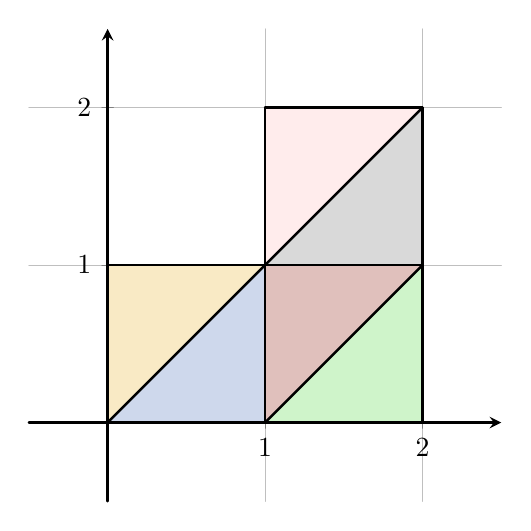
\begin{tikzpicture}[every path/.style={line cap=round, line width=0.03cm}]
		
		\begin{axis}[
			x=2.0cm,y=2.0cm,
			axis lines=middle,
			ymajorgrids=true,
			xmajorgrids=true,
			xmin=-0.5,
			xmax=2.5,
			ymin=-0.5,
			ymax=2.5,
			xtick={-6,-5,...,6},
			ytick={-3,-2,...,3},]
			
			\fill[blue,opacity=0.3] (0,0) -- (1,0) -- (1,1) -- cycle;
			\fill[yellow,opacity=0.3] (0,0) -- (0,1) -- (1,1) -- cycle;
			\fill[red,opacity=0.3] (1,0) -- (1,1) -- (2,1) -- cycle;
			\fill[green,opacity=0.3] (1,0) -- (2,0) -- (2,1) -- cycle;
			\fill[pink,opacity=0.3] (1,1) -- (1,2) -- (2,2) -- cycle;
			\fill[gray,opacity=0.3] (1,1) -- (2,1) -- (2,2) -- cycle;

			\draw (0,1) -- (2,1);
			\draw (2,2) -- (0,0);
			\draw (1,2) -- (1,0);
			\draw (1,0) -- (2,1);
			\draw (0,0) -- (2,0);
			\draw (1,2) -- (2,2);
			\draw (0,1) -- (0,0);
			\draw (2,2) -- (2,0);
		\end{axis}
	\end{tikzpicture}
\end{document} 
